%%%%%%%%%%%%%%%%%%%%%%%%%%%%%%%%%%%%%%%%%%%%%%%%%%
% MOMENTS 1960 vs. 1985 WITH VERTICAL BOUNDARIES %
%%%%%%%%%%%%%%%%%%%%%%%%%%%%%%%%%%%%%%%%%%%%%%%%%%

\begin{figure}[H]
  \caption{Father-Son Mobility: Raw Moments and Example CEFs} 
  \label{fig:moments_only}
  \begin{center}
    \begin{tabular}{ccc}
      \panel{A. Father-Son Rank-Rank Moments, 1960--69 and 1985--89} & 
      \panel{B. Two Valid CEFs for 1960-69 Birth Cohorts} \\ 
      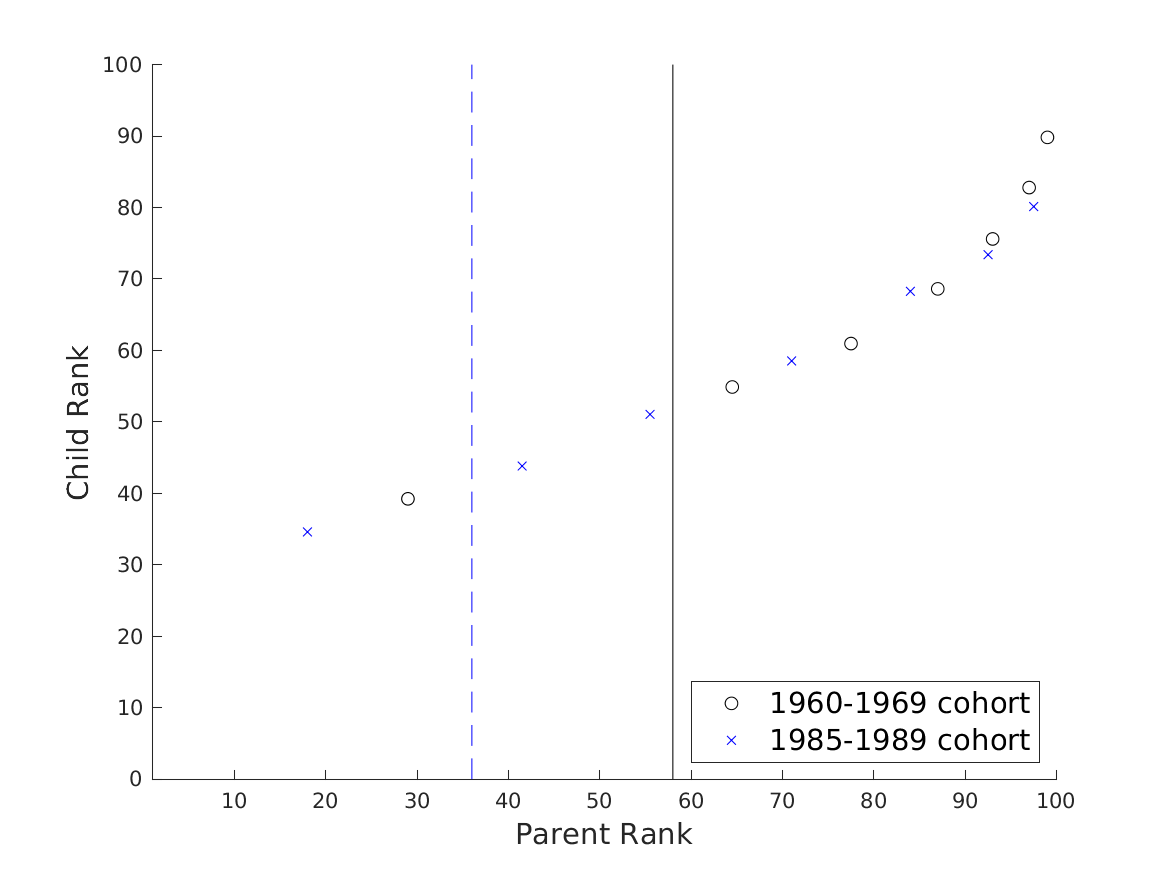
\includegraphics[scale=0.4]{\mobilitypath/moments_1960_1985.png}  & 
      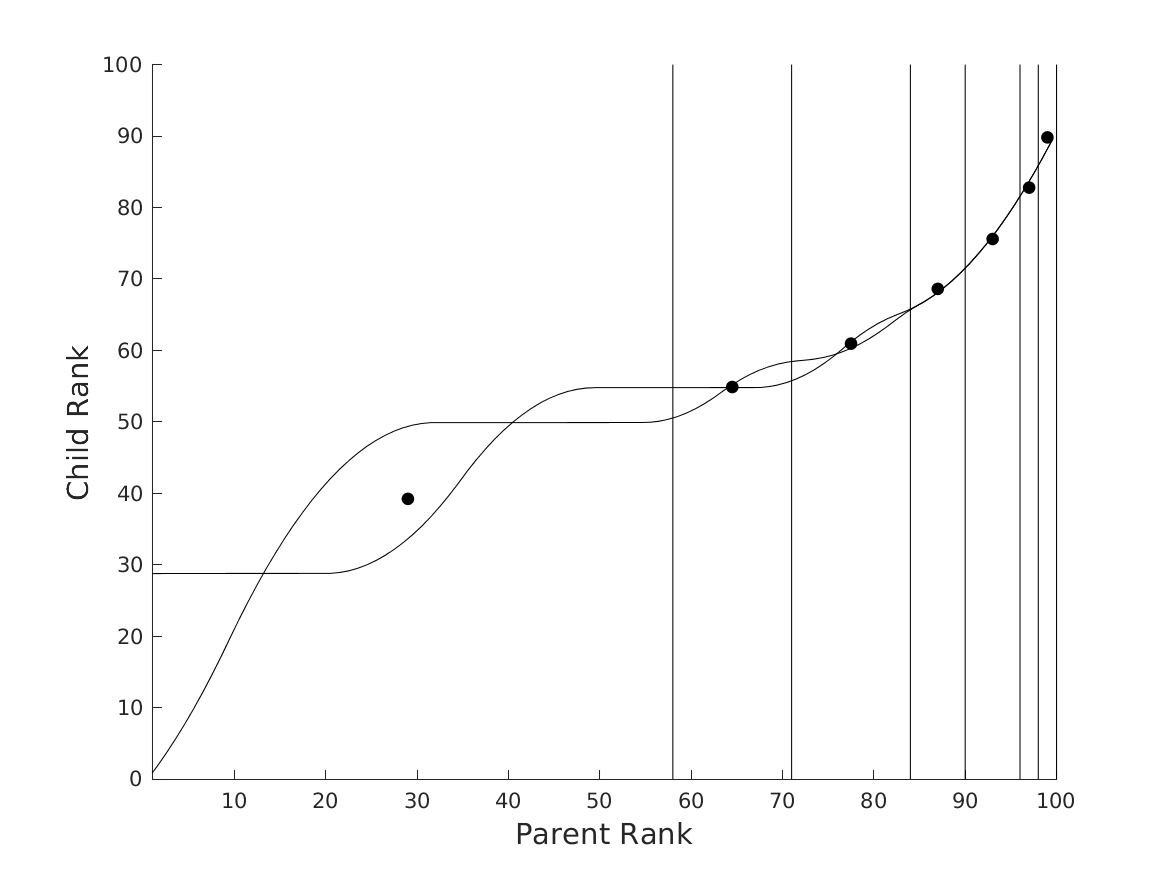
\includegraphics[scale=0.4]{\mobilitypath/fig_example_cef_1960.png} \\
\end{tabular}
\end{center}
\begin{center}
\begin{tabular}{c} 
    \panel{C. Partially Identified CEFs} \\ 
    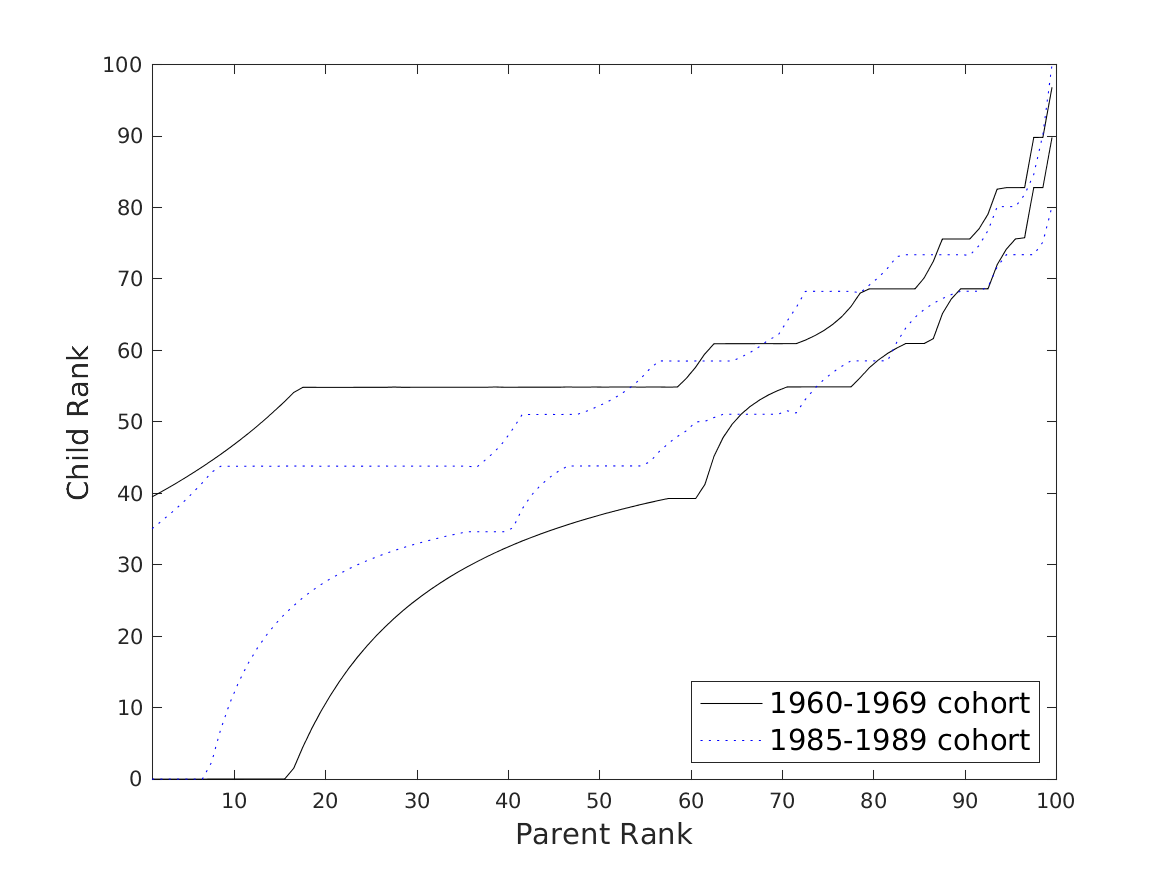
\includegraphics[scale=0.4]{\mobilitypath/fig_time_1960_25000.png}    
\end{tabular}
  \end{center}
  \newline
  \footnotesize{Panel A of the figure shows the average child
    education rank in each parent education rank bin for the 1960--69
    and 1985--89 birth cohorts. The vertical lines show the boundaries
    for the bottom parent bin, which corresponds to less than two
    years of education. The solid line corresponds to the 1960--69
    birth cohort and the dashed line to the 1985--89 birth
    cohort. Points are displayed at the midpoint of each parent
    rank bin. Panel B shows the 1960--69 moments again, along with two
    simulated conditional expectation functions which are equally good
    fits to the moments. Panel C shows bounds on father-son
  CEFs. Source: IHDS (2012).}
\end{figure}

%%%%%%%%%%%%%%%%%%%%%%%%%%%%%%%%%%%
%% ANNOTATED MU-0-50 EXPLANATION %%
%%%%%%%%%%%%%%%%%%%%%%%%%%%%%%%%%%%
\begin{landscape}
  \begin{figure}[H]
    \caption{Intuition: Calculating $\mu_0^{50}$ for 1960--69 Birth Cohort} 
    \label{fig:mu_annotation}

    \begin{center}
      \begin{tabular}{cc}
        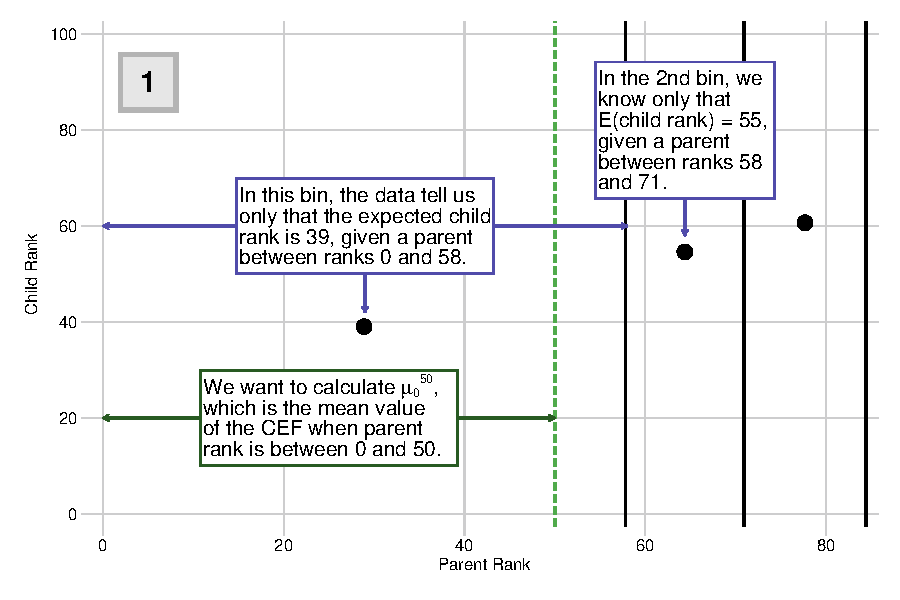
\includegraphics[scale=0.77]{\mobilitypath/example_ihds2} & 
        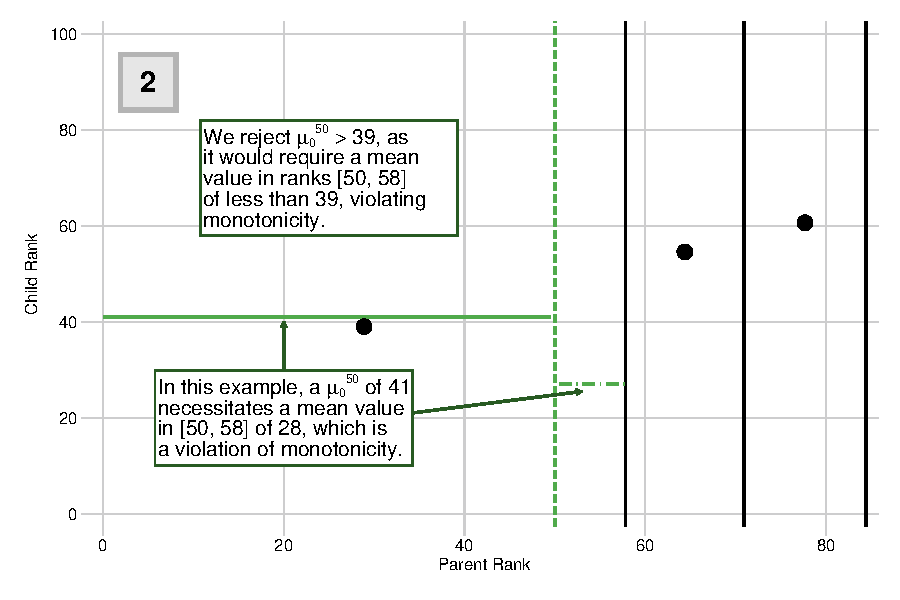
\includegraphics[scale=0.77]{\mobilitypath/example_ihds3} \\
        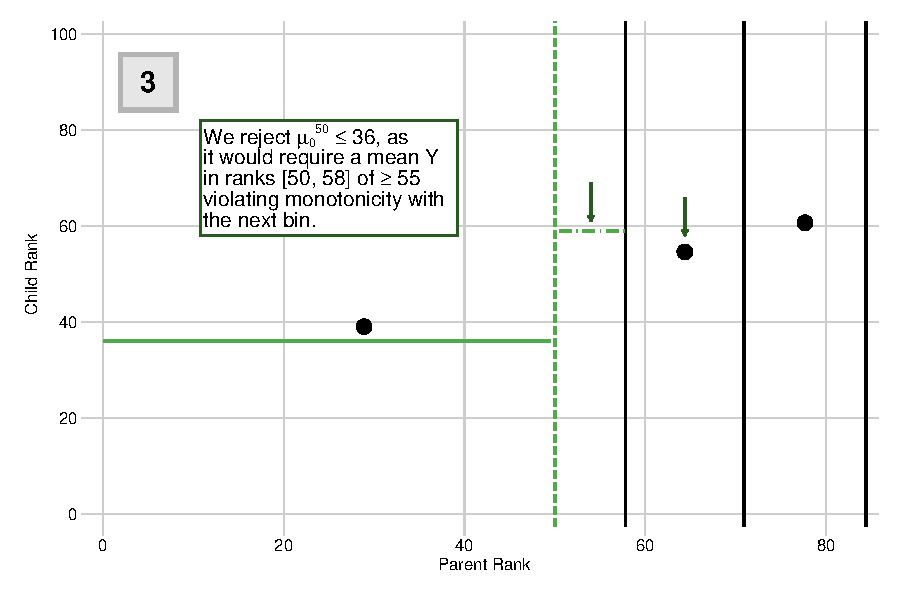
\includegraphics[scale=0.77]{\mobilitypath/example_ihds4} & 
        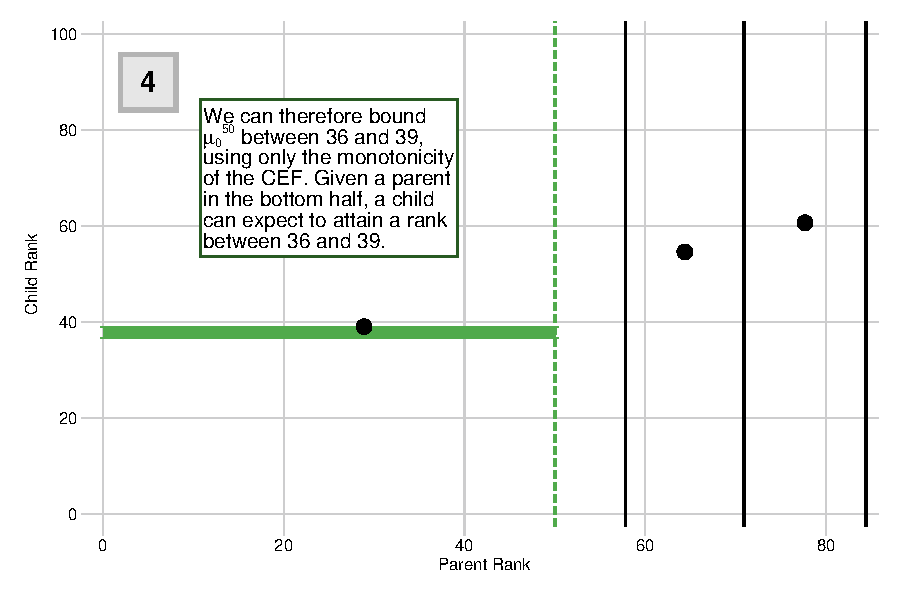
\includegraphics[scale=0.77]{\mobilitypath/example_ihds5} \\
      \end{tabular}          
    \end{center}
  \end{figure}
\end{landscape}

%%%%%%%%%%%%%%%%%%%%%%%%%%%%%%%%%%%%%
%% DESCRIPTIVE CHANGE IN EDUCATION %%
%%%%%%%%%%%%%%%%%%%%%%%%%%%%%%%%%%%%%
\begin{figure}[H]
  \caption{Changes in Educational Attainment by Birth Cohort} 
  \label{fig:descriptive_ed}
  \begin{center}
    \begin{tabular}{c} 
      \panel{A. Women} \\ 
      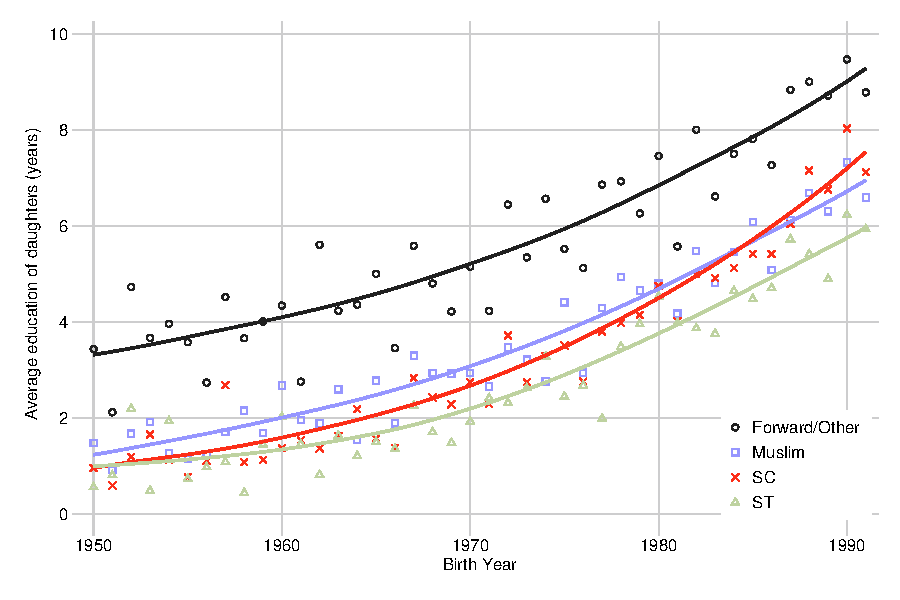
\includegraphics[scale=0.6]{\mobilitypath/daughter_ed_time} \\
      \panel{B. Men} \\ 
      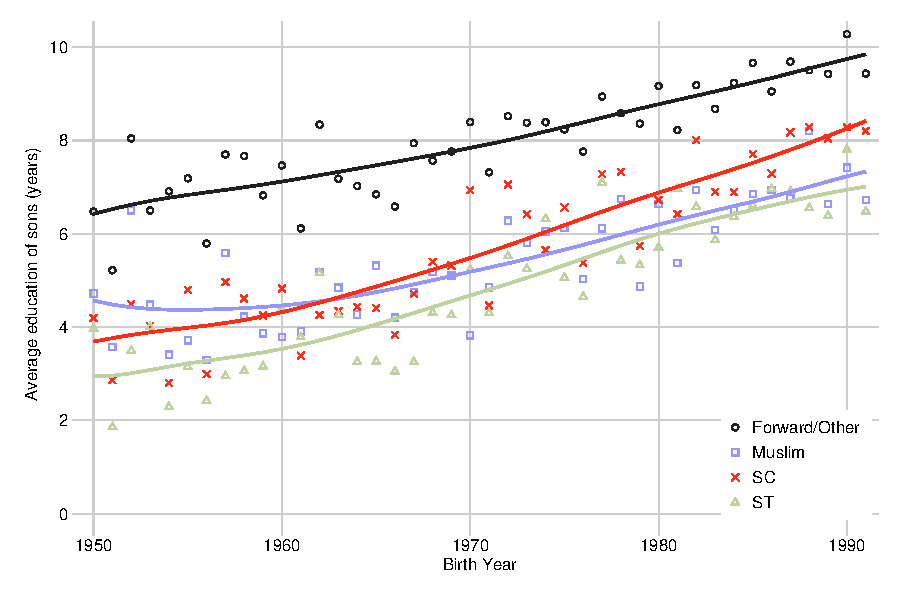
\includegraphics[scale=0.6]{\mobilitypath/son_ed_time} \\
    \end{tabular}
  \end{center}
  \footnotesize{The points show average levels of educational attainment for each birth cohort / social group. The lines are lowess curves fit to each group's time series. Source: IHDS (2012).}
\end{figure}

%%%%%%%%%%%%%%%%%%%%%%%%%%%%%%%%%%
%% BOUNDS ON p25, BETA, mu-0-50 %%
%%%%%%%%%%%%%%%%%%%%%%%%%%%%%%%%%%
\begin{landscape}
  \begin{figure}[H]
    \caption{Bounds on Father-Son Mobility Measures in India:\cnewline 1960--69 and 1985--89 Birth Cohorts}
    \label{fig:bounds_bpm}
    \begin{center}
      \begin{tabular}{ccc}
        \panel{A. Rank-Rank Gradient ($\beta$)}          &
        \panel{B. Absolute Upward Mobility  ($p_{25}$)}  &
        \panel{C. Bottom Half Mobility  ($\mu_0^{50}$)}  \\
        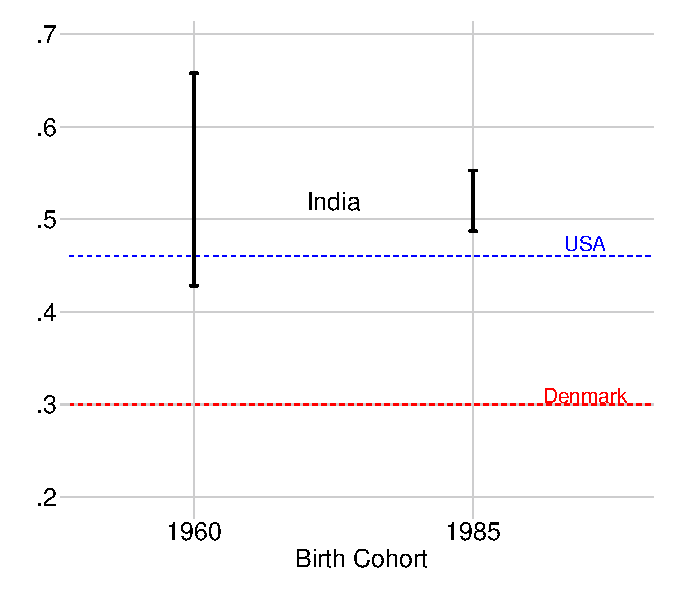
\includegraphics[scale=0.65]{\mobilitypath/gradient_60_85} &
        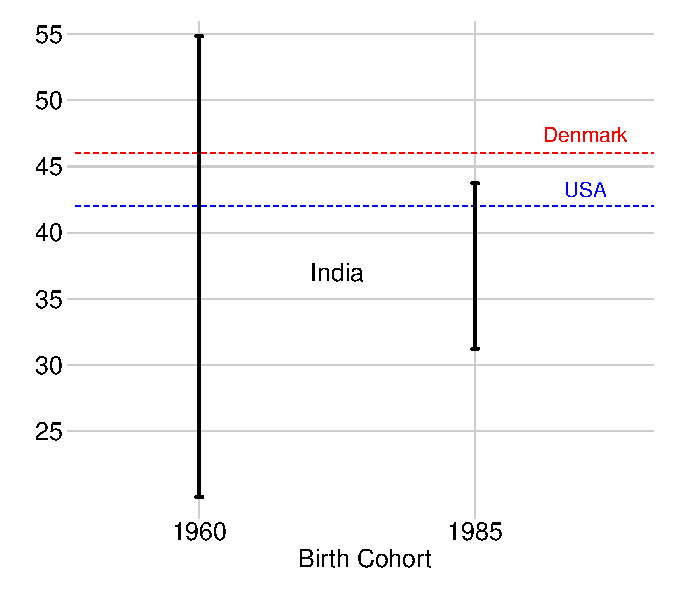
\includegraphics[scale=0.65]{\mobilitypath/p25_60_85} &
        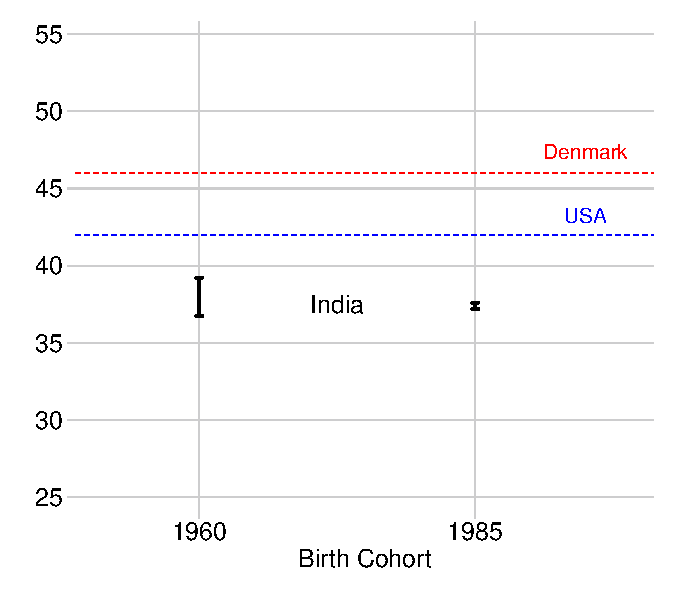
\includegraphics[scale=0.65]{\mobilitypath/mu50_60_85} \\
      \end{tabular}
      \hline
    \end{center}
    The figure shows bounds on three mobility statistics for the
    1960--69 and 1985--89 birth cohorts, estimated on father-son pairs
    in India. For reference, we display estimates of similar
    statistics from USA and Denmark. Data on rank-rank education
    gradients for USA and Denmark are from \citeasnoun{hertz2008}. For $p_{25}$ and
    $\mu_0^{50}$, the USA and Denmark references are \textit{income}
    mobility estimates from \citeasnoun{chetty2014c}. The Indian
    measures are all based on education data.  The rank-rank gradient
    is the slope coefficient from a regression of son education rank
    on father education rank. $p_{25}$ is absolute upward mobility,
    which is the expected rank of a son born to a father at the 25th
    percentile. $\mu_{0}^{50}$ is bottom half mobility, which is the
    expected rank of a son born to a father below the 50th
    percentile. Source: IHDS (2012).
  \end{figure}
\end{landscape} 

%%%%%%%%%%%
% TRENDS  %
%%%%%%%%%%%
\begin{figure}[H]
    \thispagestyle{empty}
  \caption{Bottom Half Mobility, 1950--1989 Birth Cohorts} 
  \label{fig:mu_gender}

  \begin{center}
    \begin{tabular}{cc}
      \panel{A. Father-Son Upward Mobility (Rank)}       &
      \panel{B. Father-Daughter Upward Mobility (Rank)}  \\
      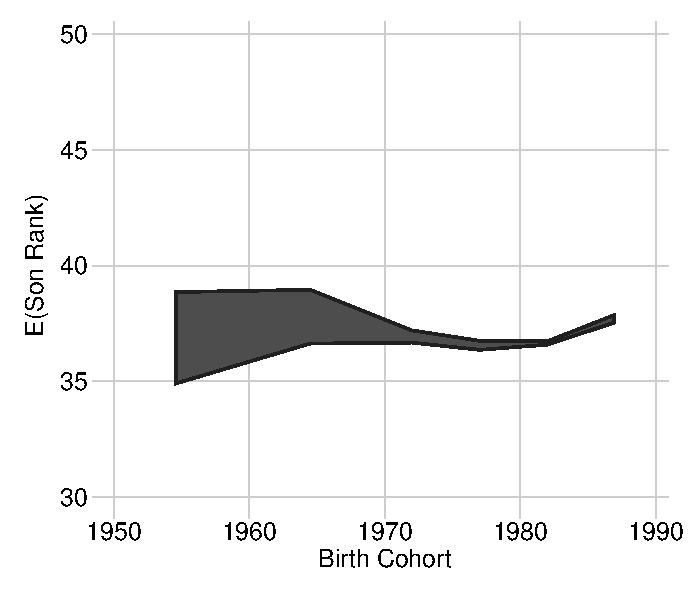
\includegraphics[scale=0.6]{\mobilitypath/ihds_mob_time_fs} &
      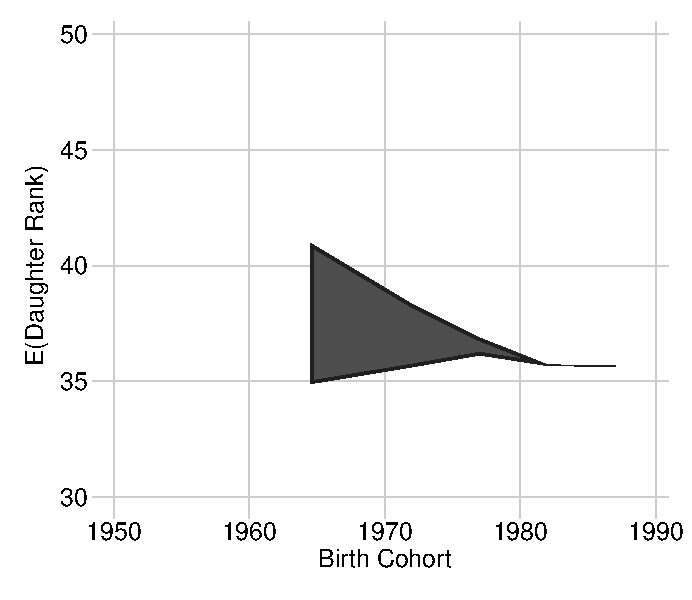
\includegraphics[scale=0.6]{\mobilitypath/ihds_mob_time_fd} \\
      \panel{C. Father-Son Mobility (Y = H.S.)} &
      \panel{D. Father-Daughter Mobility (Y = H.S.)}  \\
      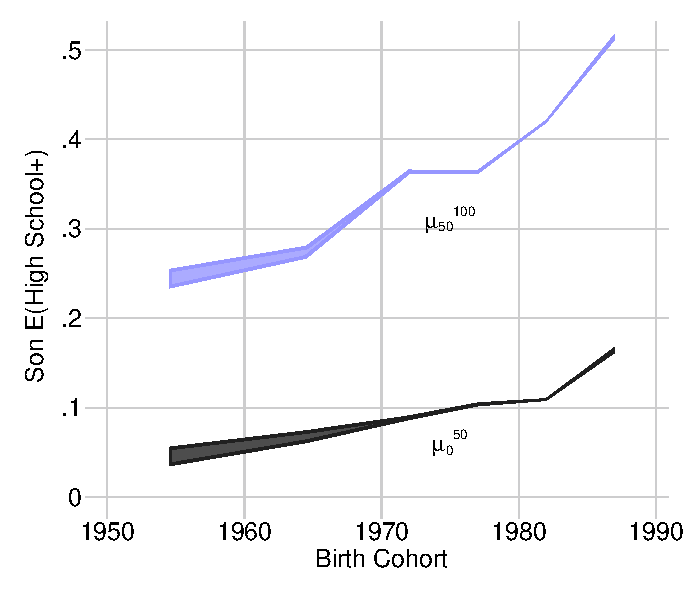
\includegraphics[scale=0.6]{\mobilitypath/ihds_mob_time_hs_m} &
      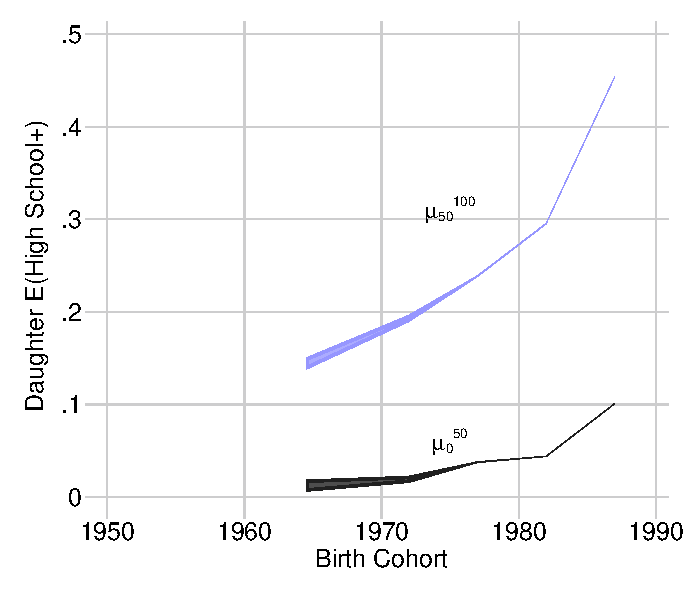
\includegraphics[scale=0.6]{\mobilitypath/ihds_mob_time_hs_f} \\
      \end{tabular}
  \end{center}

  \footnotesize{Figure \ref{fig:mu_gender} presents bounds on
    national intergenerational mobility, using cohorts born
    from 1950 through 1989. Panels A and B show bottom half mobility
    ($\mu_{0}^{50} = E(y|x \in [0, 50])$), where $x$ is parent rank and
    $y$ is child rank. This is the average rank attained by children
    born to parents who are in the bottom half of the education
    distribution, respectively for sons and daughters. Panels C and D
    show an analogous measure, $E(HS|x \in [0, 50])$ (gray) and
    $E(HS|x \in [50, 100])$ (blue). The first (gray) is the share of children
    completing high school, conditional on having parents in the
    bottom half of the education distribution. The second (blue) is the share
    of children completing high school, conditional on having parents in the
    top half of the parent distribution. Source: IHDS (2012).} 
\end{figure}

%%%%%%%%%%%%%%%%%%%%%%%%%%%%%%%%%%%%%%%%%%%%
%% TRENDS BY SOCIAL GROUP -- FATHER-CHILD %%
%%%%%%%%%%%%%%%%%%%%%%%%%%%%%%%%%%%%%%%%%%%%
\begin{figure}[H]
  \caption{Trends in Mobility by Subgroup, 1950--1989 Birth Cohorts} 
  \label{fig:group_mob}

  \begin{center}
    \begin{tabular}{cc}
      \panel{A. Father-Son Upward Mobility $\boldsymbol \mu_0^{50}$}  &
      \panel{B. Father-Son Downward Mobility $\boldsymbol \mu_{50}^{100}$}   \\
      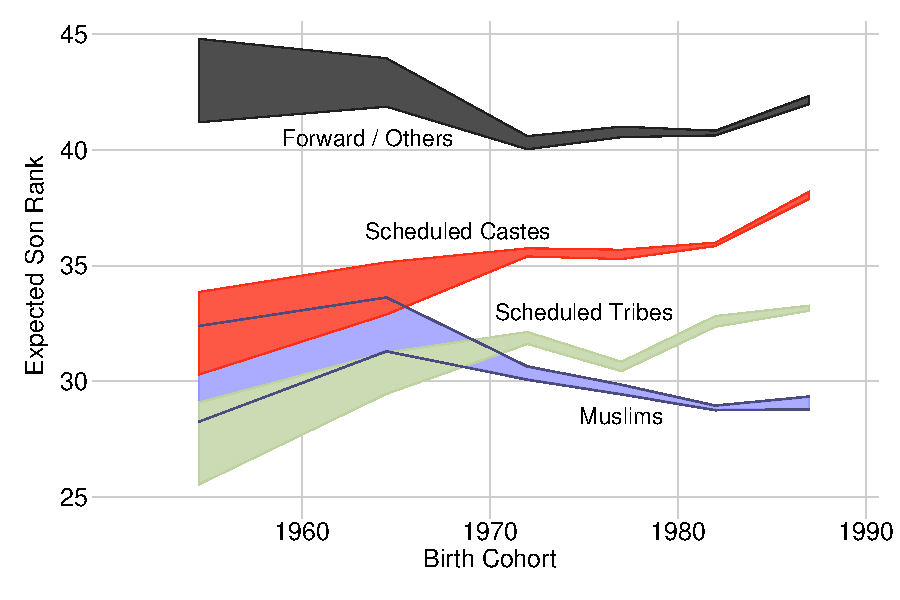
\includegraphics[scale=0.55]{\mobilitypath/ihds_mob_group_time_p25_m}
                                            & 
      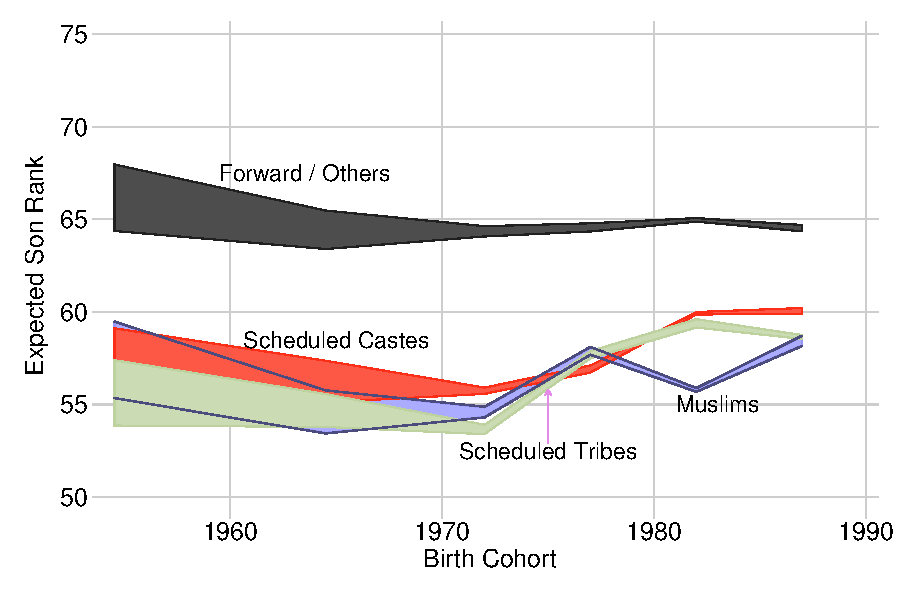
\includegraphics[scale=0.55]{\mobilitypath/ihds_mob_group_time_p75_m}  \\ 
      
      \panel{C. Father-Daughter Upward Mobility $\boldsymbol \mu_0^{50}$}  &
      \panel{D. Father-Daughter Downward Mobility $\boldsymbol \mu_{50}^{100}$}   \\
      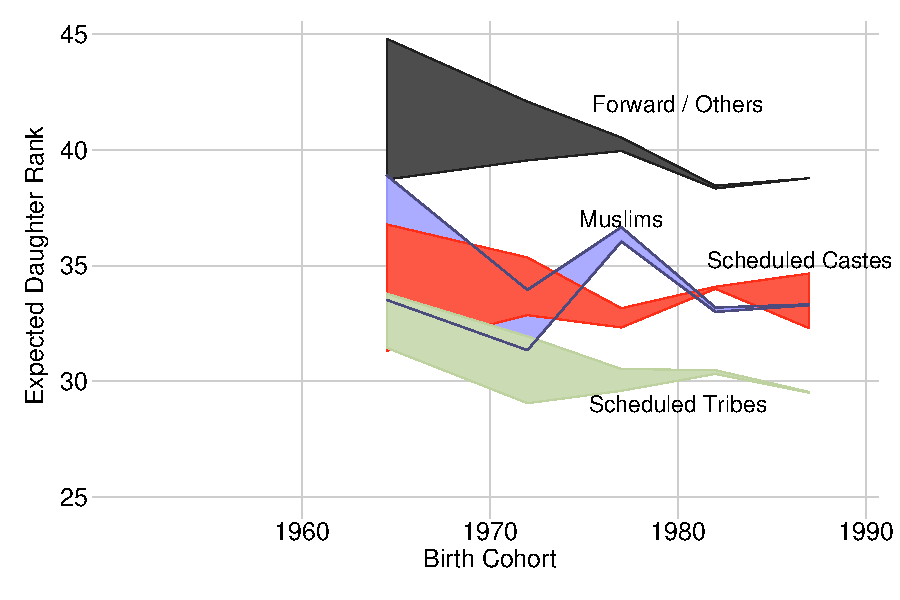
\includegraphics[scale=0.55]{\mobilitypath/ihds_mob_group_time_p25_f}
                                                 & 
      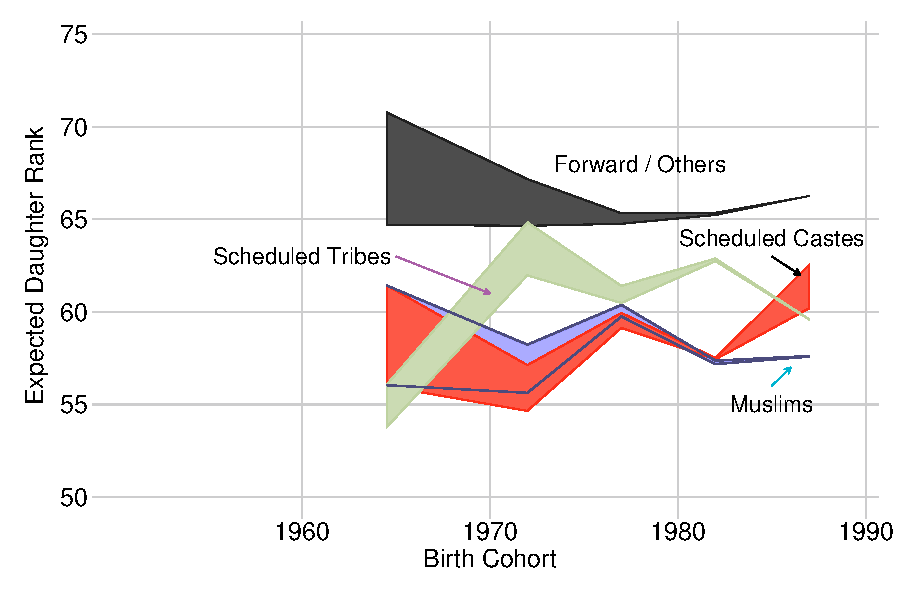
\includegraphics[scale=0.55]{\mobilitypath/ihds_mob_group_time_p75_f} \\
      \end{tabular}          
  \end{center}
  \newline
  \footnotesize{Figure~\ref{fig:group_mob} presents bounds on trends
    in intergenerational mobility, stratified by four prominent social
    groups in India: Scheduled Castes, Scheduled Tribes, Muslims, and
    Forward Castes/Others. The mobility measure in Panels A and C is
    bottom half mobility ($\mu_0^{50}$), or the average rank among
    children born to fathers in the bottom half of the father
    education distribution. The measure in Panels B and D is top half
    mobility ($\mu_{50}^{100}$), or the average rank among children
    born to fathers in top half of the father education
    distribution. Linked father-daughter education data are not
    available for the 1950--59 birth cohort.  Source: IHDS (2012).}
\end{figure}

%%%%%%%%%%%%%%%%%%%%%%%%%%%%%%%%%%
%% Affirmative action - cassan  %%
%%%%%%%%%%%%%%%%%%%%%%%%%%%%%%%%%%
\newpage 
\begin{figure}[H]
  \caption{Jati Redesignation and Intergenerational Mobility} 
  \label{fig:cassan}
  \begin{center}    
      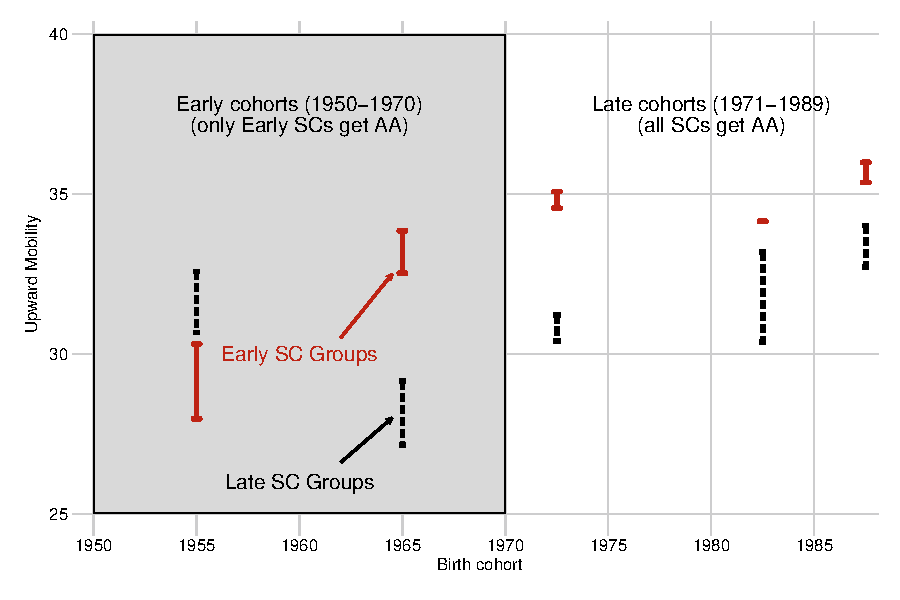
\includegraphics[scale=1.15]{\mobilitypath/jati_cohort_mob}
  \end{center}
  \newline
  \footnotesize{Figure~\ref{fig:cassan} shows bounds on bottom half
    mobility $\mu_0^{50}$ for two social groups in India. The dark red
    series shows upward mobility for groups that were designated as
    Scheduled Castes since before 1956. The black series shows
    upward mobility for groups that were not designated as Scheduled
    Castes until 1977; birth cohorts later than 1970 (outside the grey
    box) were six or younger when the policy change was implemented and thus would have had SC status at the primary school-starting age. Source: IHDS
    (2012).}
\end{figure}

